% TODO: Remove em-dashes
% This is an em-dash: —

% General notes 

% 2023-06: last observation at time of meeting
% [1] "2023-06"
% Meeting time 2023-06-14 14:00:00 
% Last observation in PM_df:  2023-06-14 14:00:16 
% Last observation in ZQ_IP_df:  2023-06-14 14:00:00 


% 2023-11 no data after meeting (PM had no further trades)
% [1] "2023-11"
% Meeting time 2023-11-01 14:00:00 
% Last observation in PM_df:  2023-10-31 12:06:41 
% Last observation in ZQ_IP_df:  2023-10-31 12:06:00 

% business largely normal elsewhere

\documentclass[a4paper,11pt]{article}
\usepackage[left=2.5cm,right=2.5cm,top=2.5cm,bottom=2.5cm]{geometry}
\usepackage[utf8]{inputenc}
\usepackage[ngerman,english]{babel}

\usepackage{amsmath}
\usepackage{amsfonts}
\usepackage{booktabs}
% \usepackage{bookmark}
\usepackage{float}
\usepackage{graphicx}
\usepackage{helvet}
\usepackage{hyperref}
\usepackage{parskip}
\usepackage{setspace}
\usepackage{svg}
\usepackage{tabularray}
\usepackage{titling}
\usepackage{xcolor}
\usepackage{caption}
\hypersetup{
    breaklinks=true,
    citecolor=black,
    colorlinks,
    filecolor=black,
    linkcolor=black,
    urlcolor=black
}
\UseTblrLibrary{booktabs}


\usepackage{natbib}
\bibliographystyle{apalike2}

% \setlength{\droptitle}{-5em}
% \onehalfspacing

\begin{document}


\newgeometry{left=2cm,right=2cm,top=2cm,bottom=2cm}

\thispagestyle{empty}
\begin{figure}[h!]
    \raggedleft
    
\includegraphics[scale=0.8]{WUlogo.pdf}
\end{figure}


\begin{center}
    \textbf{\huge MASTERARBEIT / MASTER’S THESIS} \\
    \vspace{1.5cm}
    
    Titel und ggf. Untertitel der Masterarbeit /
    Title and, if applicable, subtitle of the Master‘s Thesis \\

    \LARGE Titel/Title \\
    \vspace{2.5cm}
    
    \normalsize verfasst von / submitted by \\
    \vspace{0.5cm}
    
    \textit{\Large Peter Pavicic BSc (WU) / \\
    Peter Pavicic BSc (WU) \\
    \vspace{.5cm}
    }
    \vspace{2cm}
    
    angestrebter akademischer Grad / intended degree: \\
    \Large Master of Science (WU) / MSc (WU)
        \\
\vspace{1cm}
\normalsize

    \begin{tabular}{ll}
        Matrikelnummer / student ID number: & 11921713 \\
        Studium / degree programme: & Quantitative Finance \\
        Betreut von / Supervisor: & Assist.Prof. Dr. Felix Fattinger \\
    \end{tabular}
    \vspace{2cm}
    
    \textbf{Wien, September 2025 / Vienna, September 2025}
\end{center}




\tableofcontents
\listoffigures

\section{Introduction}

Lorem ipsum dolor sit amet, consectetur adipiscing elit. Proin nec eleifend mi, vel faucibus ligula. Suspendisse tempus fringilla elit a interdum. Nunc non placerat lectus, non aliquet turpis. Morbi id maximus lacus. Sed nec mi non erat vehicula tincidunt eget eu lorem. Nam quis urna quis justo elementum vestibulum ac finibus lectus. Vivamus congue porttitor dui maximus commodo. Nunc scelerisque enim sem, nec sodales tellus ornare quis. Sed non velit vitae massa commodo consequat. Quisque dui lorem, congue eu hendrerit nec, laoreet non arcu. Fusce sed vestibulum ligula. In in pretium nulla.

Donec neque neque, iaculis in vestibulum et, varius eget enim. Phasellus in nisi nunc. Etiam in sollicitudin libero, quis elementum elit. Ut tincidunt sem a libero viverra mattis. Phasellus ut tortor fermentum, dapibus ipsum eget, rutrum nibh. Phasellus ullamcorper pellentesque ipsum, sit amet imperdiet dui faucibus a. Praesent ullamcorper erat a leo consectetur, sit amet dictum metus accumsan. Donec in commodo purus, vitae ornare lectus. Aliquam pretium nisi eros, vitae venenatis ex egestas et. Cras varius vestibulum vestibulum. Cras efficitur ullamcorper justo ac tempor. Etiam condimentum condimentum est ut lacinia. Nullam augue massa, interdum at eros a, porttitor tincidunt felis. Duis tempor quam quis ante dignissim, sit amet lacinia sem ornare. Donec lacinia fermentum diam ut mattis.

Donec eu justo nec sem rutrum vehicula. Ut et vulputate sem. Nunc ex diam, mollis sed leo non, pulvinar sodales nulla. Mauris aliquam eros iaculis, suscipit libero ac, vehicula libero. Suspendisse potenti. In cursus diam at diam faucibus, nec fermentum sem pellentesque. Maecenas convallis fermentum mauris ut tempus. In congue nisl nisi, et consequat ligula consequat vel. Nulla non sapien nec nulla tincidunt tristique vestibulum volutpat augue. Aenean eu suscipit tellus, auctor auctor elit. Curabitur aliquam magna lacus, eu commodo purus convallis vel.

Integer mollis rutrum purus, sed mattis est consequat ac. Suspendisse potenti. Fusce egestas ornare tempor. Mauris euismod risus leo, sit amet suscipit risus rhoncus eu. Duis at varius orci. Donec purus risus, cursus blandit dolor sit amet, cursus ornare mi. Class aptent taciti sociosqu ad litora torquent per conubia nostra, per inceptos himenaeos. Vestibulum vitae tempor ligula, at placerat felis. Duis in condimentum ante, nec accumsan lacus. Mauris vehicula nisl eget orci ornare placerat. Nam molestie mi nisl, id luctus lorem commodo quis. Fusce iaculis lectus sodales nulla fermentum convallis. Phasellus aliquam urna ut lectus hendrerit facilisis.

Nunc ut magna ullamcorper, consequat erat sed, tristique libero. Proin rhoncus vulputate nisl, eu interdum massa maximus quis. In luctus enim vel cursus scelerisque. Orci varius natoque penatibus et magnis dis parturient montes, nascetur ridiculus mus. Sed at facilisis justo. Etiam sit amet pulvinar felis. Vivamus nibh massa, tempus vulputate ipsum nec, vulputate aliquam nunc. Morbi quis enim purus. Etiam congue magna vitae ultricies cursus. Aliquam erat volutpat. Curabitur tincidunt suscipit iaculis. Aliquam eu tellus molestie, dignissim felis ut, finibus leo. Quisque in eros est. 





\section{Theoretical Framework}

% TODO: Humanise
\subsection{Prediction Markets} \label{sec:prediction_markets}

Prediction markets are financial markets designed to forecast future events. Participants of prediction markets trade state-contingent claims whose payoff depends on how those future events unfold.
While different types of prediction markets have been designed, the scope of this thesis is limited to winner-take-all prediction markets. These markets are typically structured in the following way: a claim costs $\$p$ today and pays $\$1$ if and only if the stated event occurs, and $\$0$ otherwise. This structure implies two participants agreeing on the price $\$p$ which one of the participants pays, the other putting up $\$(1 - p)$, with the winner receiving "all" of the dollar put up in collateral as their payoff. \citep{wolfers_prediction_2004}. 
% Arrow-Debreu securities? 
% The price $p$ can be read as the market-implied (risk-neutral) probability that the event happens, because the contract’s expected payoff equals p. Put differently, the price is a state price; under standard assumptions it coincides with the event’s probability. The same logic underlies families of related contracts (for example, across thresholds or outcomes), whose internal consistency and co-movement reflect how new information is incorporated through trading.

Through price discovery, traditional financial markets aggregate information about the value of assets. Prediction markets’ primary purpose is leveraging this role of markets for forecasting. Under the Efficient Markets Hypothesis, the market price on prediction markets should reflect the risk-neutral probabilities of the event in question, encompassing all available information.
\citep{berg_prediction_2008}


% A winner-take-all example makes this concrete. Suppose there is a market on an election between two candidates, A and B. The contract “A wins” pays \$1 if A is elected, \$0 otherwise; likewise for “B wins.” In equilibrium, the “YES” price on A (say 0.62) is the market’s risk-neutral probability that A will win (62\%), and the “YES” price on B will be close to 1 - 0.62 = 0.38. If the two “YES” prices do not sum to one, arbitrageurs can buy the underpriced side(s) or sell the overpriced side(s) until prices realign, restoring probabilistic coherence and reinforcing information aggregation.
% Cite Wolfers and Zitzewitz
% Cite Seguillo


% In short, prediction markets function by turning beliefs about uncertain events into tradable payoffs; if EMH holds even approximately, the resulting prices are interpretable as expected values—risk-neutral probabilities in winner-take-all settings—making platforms like Polymarket natural objects for empirical study of price discovery.
% % Cite Wolfers and Zitzewitz
% % Cite Seguillo



% NOTE: Move to literature review or write literature review here?
% TODO: Elaborate
This efficiency and predictive power of prediction markets has been the topic
of vast existing literature, especially in the context of forecasting elections, such as in
\cite{berg_prediction_2008} \cite{erikson_are_2008}, who have found that .... 
% Empirical Berg (2008)
% Analytical Wolfers (2006)
This has also been tackled analytically, where \cite{wolfers_interpreting_2006} derived two economic models which
describe sufficient conditions under which prediction markets prices correspond with participants' mean beliefs.
% Prediction markets were originally started by the Iowa State University for the 1988

% TODO: Write segue
However, little research has been done examining the world's largest prediction market as of 2025, Polymarket.
This is thesis aims to provide empirical research into the market efficiency of winner-take-all prediction markets 
in the context of markets focusing on the interest rate decisions of the US Federal Open Market Committee's (FOMC) following their scheduled meeting.

% TODO: Remove this when previous section written
\newpage

\subsection{Polymarket}


\subsubsection{Concepts and terminology}
Polymarket is the world's largest prediction market-hosting platform, % todo: Source?
hosted on the website www.polymarket.com.
% Figure % todo: Create and reference figure
% depicts the front page as taken on September 3rd, 2025.

% Figure out how to put this image where I want it to be
\begin{figure}[H]
  \begin{center}
    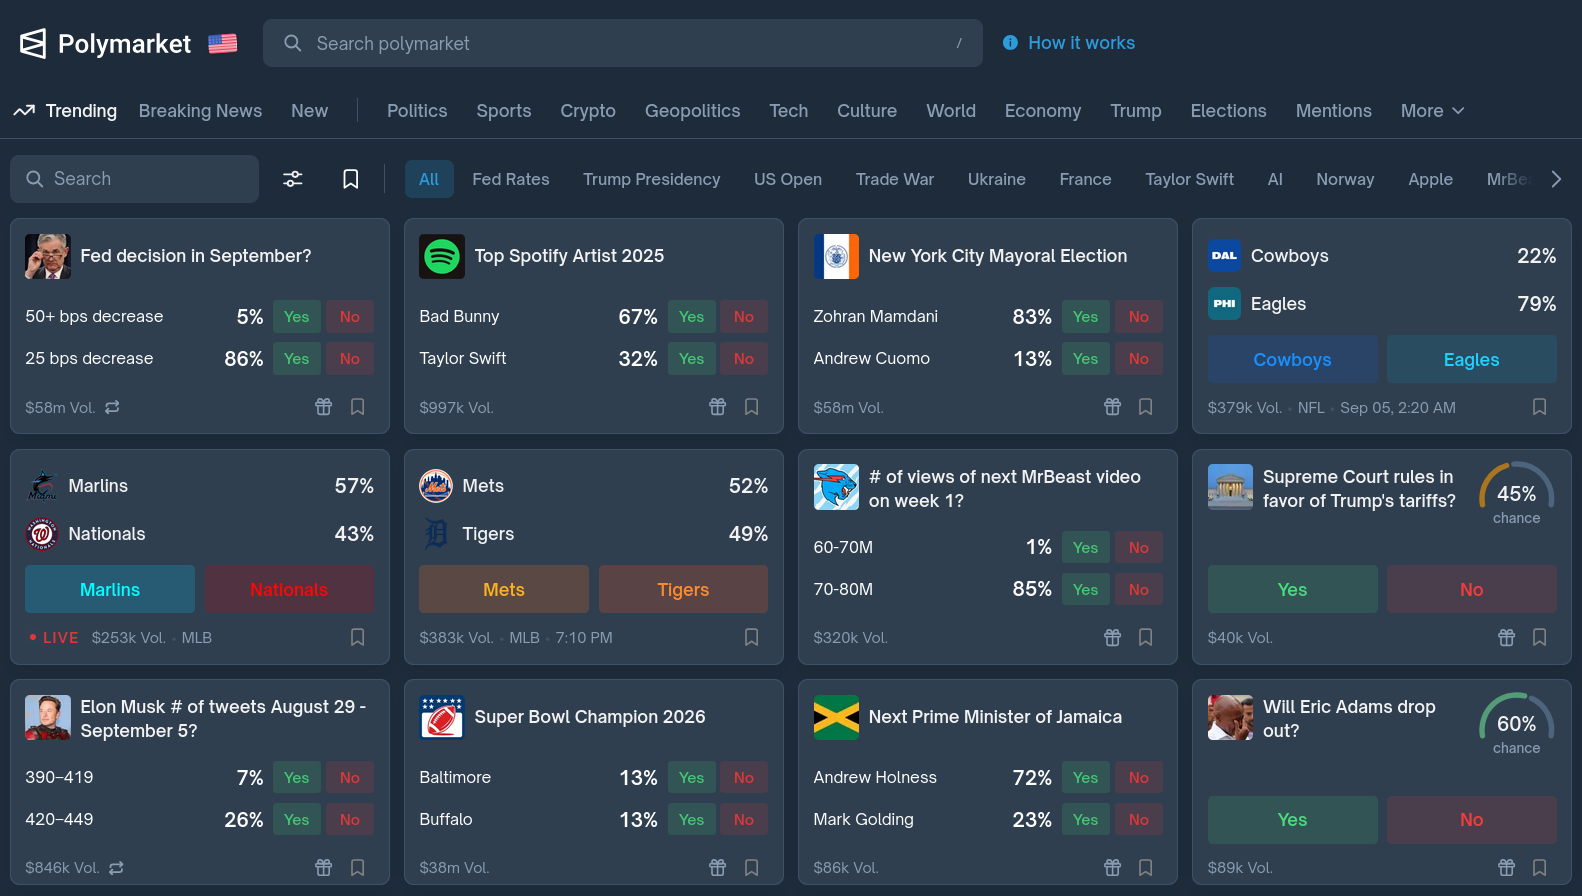
\includegraphics[width=0.95\textwidth]{figures/Polymarket_front_page.png}
  \end{center}
  \caption{The Polymarket front page as of September 3rd, 2025. While there is a variety of events, sports and politics markets are among the most popular}
  % \label{fig:front_page}
\end{figure}


On Polymarket, prediction markets are grouped into "events", which contain "markets" related to a single topic/occasion.
Each "market" is a winner-take-all market as outlined in Section \ref{sec:prediction_markets}. For each listed market, there are two complementary outcomes, labeled Yes and No with prices between \$0 and \$1.


% Figure % todo: Insert figure and reference it
% depicts the Polymarket event for the interest rate decision of the FOMC following their scheduled September meeting.

% Caption: Each market related to a possible decision (50 bps increase, 25 bps decrease, no change, etc.) related to a single FOMC meeting is grouped into 


% Figure out how to put this image where I want it to be
\begin{figure}[H]
  \begin{center}
    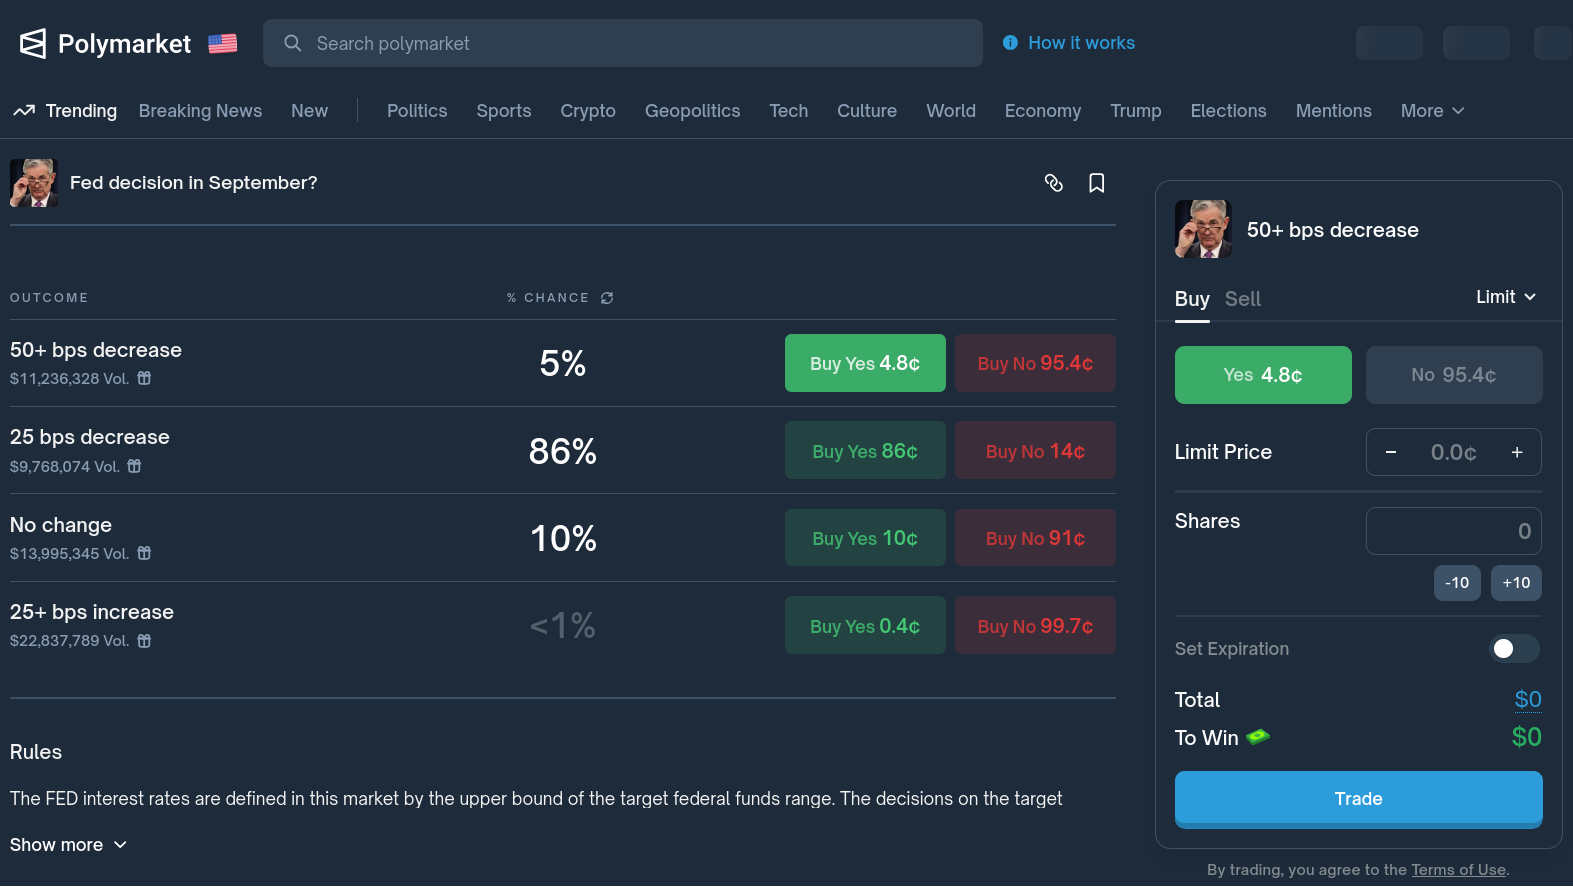
\includegraphics[width=0.95\textwidth]{figures/FOMC_event_September.png}
  \end{center}
  \caption{September FOMC event on Polymarket as of September 3rd, 2025}
  % FIX: this
  \caption*{kjansdkjnakjdnasjkdnakjdnaskjdasndjkn}
  % \label{fig:front_page}
\end{figure}


\subsubsection{design: Yes/No assets, central limit order book, and full collateralization}

%%%%%%%%%%% UNREVIEWED TEXT STARTS HERE %%%%%%%%%%%

Trading occurs on a centralized limit order book operated off-chain with on-chain settlement. Participants submit limit orders to buy or sell Yes or No claims at chosen prices; an operator matches orders and submits matched trades to an exchange smart contract that atomically swaps collateral for outcome tokens. Because the order book is continuous and open throughout the market’s life, traders can enter, exit, and revise positions at any time, and prices update in real time as new orders arrive. With two-sided liquidity, standard market microstructure logic applies: supply and demand determine the sequence of matches, and under informational efficiency, the trading process aggregates dispersed signals into prices that serve as real-time forecasts. ([Polymarket Documentation][2])

Contracts are fully collateralized at issuance and throughout trading by design. Operationally, one unit of collateral can be “split” into a full set consisting of one Yes and one No token for the same condition, ensuring that the sum of outcome shares is always backed by 1 unit of collateral that will be released to the eventual winner. Symmetrically, a holder of a full set can “merge” the tokens to reclaim collateral. At resolution, holders of the winning outcome burn their tokens to redeem the embedded collateral. This split/merge/redeem triad enforces the accounting identity behind the no-arbitrage relation $P_{\text{Yes}} + P_{\text{No}} = 1$ and guarantees performance of payoffs at resolution. ([Polymarket Documentation][3])


% Figure out how to put this image where I want it to be
\begin{figure}[H]
  \begin{center}
    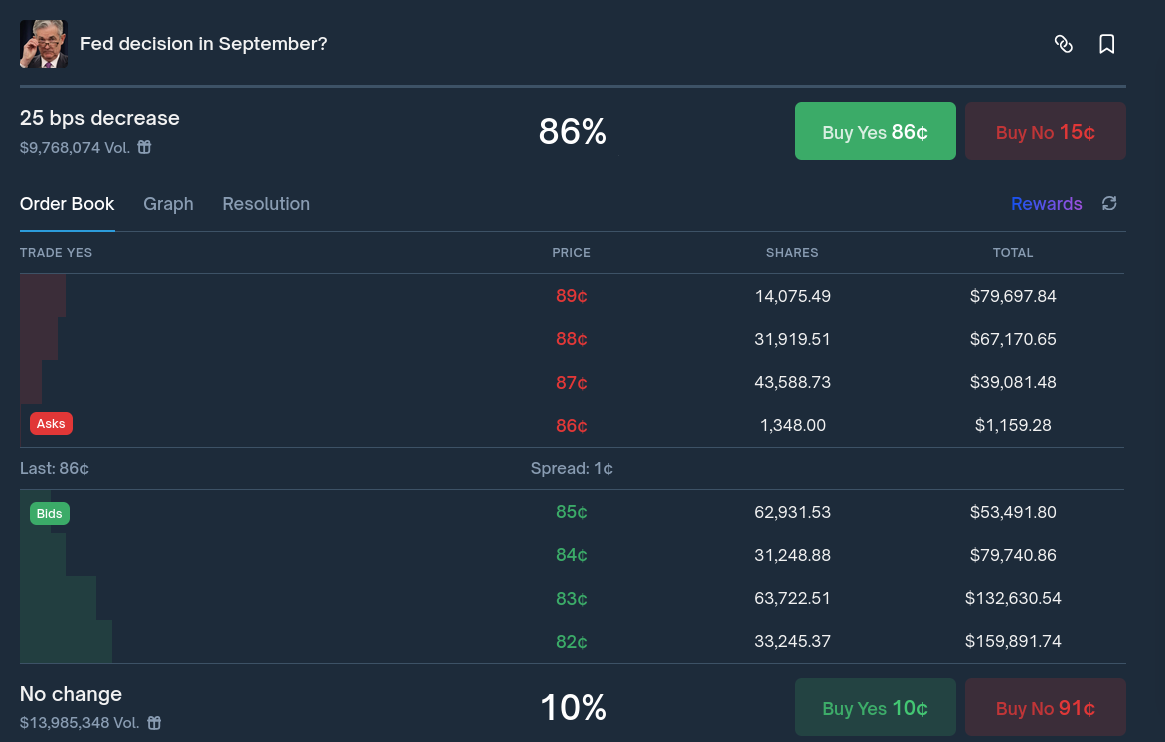
\includegraphics[width=0.95\textwidth]{figures/polymarket_continuous_double_auction.png}
  \end{center}
  \caption{The Polymarket front page as of September 3rd, 2025. While there is a variety of events, sports and politics markets are among the most popular}
  % \label{fig:front_page}
\end{figure}

\subsubsection{discovery and informational interpretation}

In this structure, each order expresses a view about mispricing of a contingent payoff. When public or private information arrives, informed traders buy underpriced outcomes or sell overpriced ones; their orders move the best quotes and, when matched, move the last trade. Under the efficient markets hypothesis, the price sequence forms a martingale with respect to the market’s information filtration, and the level of the Yes price is an efficient forecast of the event’s risk-neutral probability. The hybrid design does not change the economic logic: the off-chain order book determines matching and the on-chain settlement guarantees delivery, but the informational content is determined by competition among heterogeneous beliefs. The platform’s own presentation of prices as probabilities is consistent with this theoretical interpretation and with empirical evidence that prediction markets aggregate information effectively. ([Polymarket Documentation][4])

\subsubsection{matching mechanics and the linkage between Yes and No}

Beyond standard maker–taker matches in a single line of the book, Polymarket’s exchange contract implements order-level logic that ties the two complementary tokens together so the full-set accounting holds at execution. As documented by Saguillo, Ghafouri, Kiffer and Suarez-Tangil (2025), there are three economically distinct pathways by which orders get matched and settled:

Direct trade. A taker’s marketable limit order in a given outcome token matches resting maker orders on the same side of the market. Settlement is a straightforward token-for-collateral swap at the matched price(s). On-chain, these fills are recorded as OrderFilled events. This is the pure order-book mechanism familiar from equities, and it governs most routine executions. ([arXiv][5])

Mint via PositionSplit. Because complementary outcomes must sum to one dollar of collateral, the exchange can also satisfy opposite-side demand across the two books by minting a new full set. When a buy order for Yes at price $p$ meets a buy order for No at price $1-p$, the contract locks 1 unit of collateral and mints one Yes and one No token, delivering each to the respective buyer. Economically, this is equivalent to sourcing inventory from the collateral pool rather than from an external holder. On-chain, the mint is captured by a PositionSplit event alongside OrderFilled events for the two sides. This pathway helps keep the two order books coupled and supports tight complementary pricing even when inventory on one side is scarce. ([arXiv][5], [Polymarket Documentation][3])

Burn via OrdersMerged. The reverse operation retires a full set and releases collateral when aggregate sell orders across the two books sum to one dollar. For example, simultaneous sells of Yes at $p$ and No at $1-p$ allow the contract to burn the pair of tokens and return 1 unit of collateral to the sellers’ counterparties, recording an OrdersMerged event together with the corresponding OrderFilled events. Economically, this drains inventory back into the collateral pool and enforces the accounting constraint in the face of two-sided liquidation pressure. ([arXiv][5], [Polymarket Documentation][6])

These three execution paths are complementary: the direct trade path matches inventory held by other users; the PositionSplit path manufactures fresh inventory when demand is balanced across the complementary books; and the OrdersMerged path retires inventory when supply is balanced. Each path preserves the invariant that a Yes and a No for the same condition are worth, in combination, exactly one unit of collateral at issuance and prior to resolution. The platform’s order-book and API documentation reflect the maker–taker structure and the unified handling of complementary tokens, while independent data sources expose these mechanics through emitted events such as OrdersMatched at the taker level and OrderFilled/OrdersMerged at settlement. ([Polymarket Documentation][2], [Goldsky][7])

\subsubsection{inventory transformations and their implications}

Crucially, the split/merge operations are not restricted to matching engine internals; users may proactively split collateral into a full set or merge a full set back into collateral at any time after a condition is prepared. This enables inventory management and hedging strategies familiar from contingent-claim markets. A trader who wants to make a market can mint full sets to provision inventory on both sides; a trader who has accumulated offsetting Yes and No across executions can merge to crystallize collateral and compress balance-sheet usage. At the microstructure level, these user-driven transformations add elasticity to supply on both sides of the book, which, in turn, tightens complementary pricing and facilitates efficient price discovery. In combination with the three settlement pathways, they make explicit the tight coupling between the books for Yes and No and operationalize the economic identity that one unit of collateral underlies the pair. ([Polymarket Documentation][3])

\subsubsection{and redemption}

% Put this where redemption is explained


% September market rules
\begin{quote}
  {
    \raggedright
    The FED interest rates are defined in this market by the upper bound of the target federal funds range. The decisions on the target federal fund range are made by the Federal Open Market Committee (FOMC) meetings.

    This market will resolve to the amount of basis points the upper bound of the target federal funds rate is changed by versus the level it was prior to the Federal Reserve's September 2025 meeting.

    If the target federal funds rate is changed to a level not expressed in the displayed options, the change will be rounded up to the nearest 25 and will resolve to the relevant bracket. (e.g. if there's a cut/increase of 12.5 bps it will be considered to be 25 bps)

    The resolution source for this market is the FOMC’s statement after its meeting scheduled for September 16 - 17, 2025 according to the official calendar:
    % \linebreak
    https://www.federalreserve.gov/monetarypolicy/fomccalendars.htm.

    The level and change of the target federal funds rate is also published at the official website of the Federal Reserve at
    % \linebreak
    https://www.federalreserve.gov/monetarypolicy/openmarket.htm.

    This market may resolve as soon as the FOMC’s statement for their September meeting with relevant data is issued. If no statement is released by the end date of the next scheduled meeting, this market will resolve to the "No change" bracket. 
  }
\end{quote}

When the designated oracle finalizes the event’s outcome, the winning side is set to a payout of 1 while the losing side’s payout is 0. Holders of the winning token redeem by burning their positions for collateral via the contract’s redeem function. Because the system remained fully collateralized ex ante, there is no gap risk at resolution; the accounting identity closes as collateral is released to the winner and all losing tokens expire. This completes the contingent-claim lifecycle from issuance, through trading and inventory transformations, to settlement and redemption. ([Polymarket Documentation][8])


%%%%%%%%%%% UNREVIEWED TEXT ENDS HERE %%%%%%%%%%%





% TODO: Humanise
\subsection{Polymarket}



% \subsubsection{claims and probabilistic pricing}
%
%
% ## Summary
%
% Polymarket can be read entirely through the lens of contingent-claim pricing and order-driven microstructure. Yes and No outcome claims are fully collateralized complements whose prices add to one and whose Yes price is the market’s risk-neutral probability of the event. A hybrid CLOB matches orders continuously, with three settlement pathways-direct trade, mint via PositionSplit, and burn via OrdersMerged—tying the complementary books together. Users themselves can split and merge full sets, adding supply elasticity and aiding price alignment. Under standard efficiency assumptions, this design delivers real-time price discovery in the form of probability-like prices that aggregate dispersed information about future events. ([Polymarket Documentation][2], [arXiv][5])
%
% [1]: https://docs.polymarket.com/polymarket-learn/FAQ/what-are-prediction-markets?utm_source=chatgpt.com "What is a Prediction Market?"
% [2]: https://docs.polymarket.com/developers/CLOB/introduction?utm_source=chatgpt.com "CLOB Introduction"
% [3]: https://docs.polymarket.com/developers/CTF/split?utm_source=chatgpt.com "Splitting USDC"
% [4]: https://docs.polymarket.com/polymarket-learn/trading/how-are-prices-calculated?utm_source=chatgpt.com "How Are Prices Calculated?"
% [5]: https://arxiv.org/html/2508.03474v1 "Unravelling the Probabilistic Forest: Arbitrage in Prediction Markets"
% [6]: https://docs.polymarket.com/developers/CTF/merge?utm_source=chatgpt.com "Merging Tokens"
% [7]: https://goldsky.com/blog/polymarket-dataset?utm_source=chatgpt.com "Announcing: Polymarket Datasets Available Now - Goldsky"
% [8]: https://docs.polymarket.com/developers/CTF/redeem?utm_source=chatgpt.com "Reedeeming Tokens"


% TODO: Humanise
\subsection{Federal Funds Rate futures}

\subsubsection{Effective Federal Funds Rate (EFFR)}

The effective federal funds rate is the transaction-volume-weighted median interest rate on unsecured overnight loans of reserve balances between depository institutions in the United States. The Federal Reserve Bank of New York computes the EFFR from FR 2420 transactional reports and publishes it for the prior business day at approximately 9:00 a.m. New York time. This benchmark rate is the underlying reference for CME’s 30-Day Federal Funds futures.
% TODO: Add citation for fed article describing EFFR
% \cite{FED OF New York}

\subsubsection{Price quoting and the implied monthly average}

CME 30-Day Federal Funds (ZQ) futures are quoted in IMM index terms, with price equal to 100 minus the market-implied arithmetic average of daily EFFR over the contract’s calendar month. If the futures price for month T is $P_t^T$ (percent), the implied expected monthly average is

$$\mathbb{E}_t[\overline{r}_T] = 100 - P_t^T$$

where $\overline{r}_T$ denotes the arithmetic average of daily EFFR realizations during month $T$. This mapping follows directly from the contract’s price quotation and settlement definition. 
% TODO: add citation for CME group's FedWatch methodology tool


\subsubsection{High-level assumptions for extracting probabilities}

To translate ZQ prices into probabilities of FOMC outcomes, the CME FedWatch methodology adopts three core assumptions.

First, rate changes occur in uniform 25-basis-point increments and the EFFR adjusts proportionally to the target change.

Second, within a meeting month, the EFFR is piecewise constant: it equals a pre-meeting level up to the decision’s effective date, and a post-meeting level thereafter.

Third, anchor months without FOMC meetings pin down a month-end/start-of-next-month level that is used to propagate boundary conditions through adjacent months. Under these assumptions, ZQ prices encode a risk-neutral expectation of the path of EFFR that can be decomposed into before/after segments in meeting months and rolled across months via anchors.
% TODO: add citation for CME group's FedWatch methodology tool

\subsubsection{Anchor months and boundary conditions}

In any month with no scheduled FOMC meeting, the entire calendar month is governed by a single policy regime, so the ZQ-implied average equals the expected EFFR throughout the month. FedWatch uses these months as anchors: for an anchor month $T$,

$$\text{EFFR(End)}_{T-1}=\text{EFFR(Avg)}_{T}=\text{EFFR(Start)}_{T+1}$$

Operationally, one identifies the nearest full non-meeting month, reads $\text{EFFR(Avg)}_{T}=100-P^T$ from its ZQ price, sets the end of the prior month and the start of the following month to that level, and then propagates these boundary values backward and forward as needed when solving adjacent meeting months. This anchoring step provides the initial conditions for the system of month-by-month equations.
% TODO: add citation for CME group's FedWatch methodology tool

\subsubsection{Meeting months and the time-weighting identity}

Consider a meeting month $T$ with $m_T$ calendar days and $k_T$ days before the policy change becomes effective. Let $r_T^{-}$ denote the pre-meeting EFFR level and $r_T^{+}$ the post-meeting level. Because the futures price reflects the arithmetic monthly average, the implied average satisfies the time-weighting identity

$$\mathbb{E}_t[\overline{r}_T] = \omega_T\, r_T^{-} + (1-\omega_T)\,\mathbb{E}_t[r_T^{+}], \qquad \omega_T \equiv \frac{k_T}{m_T}
$$

Solving for the expected post-meeting level gives

$$\mathbb{E}_t[r_T^{+}] = \frac{m_T\,\mathbb{E}_t[\overline{r}_T] - k_T\, r_T^{-}}{m_T-k_T}$$

When the following month $T{+}1$ is an anchor, $\mathbb{E}_t[r_T^{+}]$ is identified directly from $\text{EFFR(Avg)}_{T+1}$. On the other hand, if the prior month is an anchor, $\,r_T^{-}$ is identified from $\text{EFFR(Avg)}_{T-1}$. In either case, the time-weighting identity links the observable ZQ-implied monthly average to the unobservable post-meeting level and enables sequential solution across the term structure. 
% TODO: add citation for CME group's FedWatch methodology tool

\subsubsection{Probability calculations via the characteristic–mantissa method}

Define the expected change in EFFR over the meeting month as $\Delta_T^{*} \equiv \mathbb{E}_t[r_T^{+}] - r_T^{-}$. Express this in units of 25 bps, $\,n_T^{*} \equiv \Delta_T^{*}/0.25\%$. Decompose $n_T^{*}$ into its characteristic (integer) and mantissa (fractional) parts:

$$
n_T^{*} = n_T + y_T,\qquad n_T \in \mathbb{Z}_{\ge 0}, 0 \le y_T < 1.
$$

FedWatch interprets this as two mutually exclusive outcomes at the meeting: a change of $n_T \times 25$ bps with probability $1-y_T$, and a change of $(n_T{+}1)\times 25$ bps with probability $y_T$. When the expected change is less than one increment ($n_T=0$), this reduces to the familiar binomial case of no change versus a single 25-bp move with probabilities $1-y_T$ and $y_T$, respectively. In the special case where the next month is an anchor and one wishes to ask only “hike or hold by 25 bps,” the implied probability collapses to

$$
\mathbb{P}(\text{25 bp hike}) 
= \frac{\text{EFFR(End)}_{T}-\text{EFFR(Start)}_{T}}{0.25\%},
\qquad 
\mathbb{P}(\text{hold})=1-\mathbb{P}(\text{hike}),
$$




% TODO: Humanise
\section{Data}

\subsection{Polymarket} \label{sec:polymarket_data}



% # Data: Sources, Construction, and Preparation

This section documents the data used in the study and the procedures by which it was collected, curated, and prepared for analysis. The empirical setting is the sequence of Federal Open Market Committee meetings for which a corresponding Polymarket contract existed. For each meeting, the core object is a paired intraday dataset comprising a Polymarket price panel and a matched panel derived from 30-Day Federal Funds Rate futures (ZQ). The emphasis here is on precise definition of the observational unit, provenance and structure of the raw data, inclusion and exclusion rules, harmonization across sources, and the measures taken to ensure reproducibility while acknowledging the limitations inherent in partly manual data assembly.

\subsection{design and unit of analysis}

The unit of analysis is an event window anchored on a single scheduled FOMC decision. For each meeting, the observation period is defined to be the lifespan of the corresponding Polymarket market, beginning at market inception and ending upon resolution at the announcement. Within each window, two time series are constructed and then aligned. The first is a panel of Polymarket outcome token prices at intraday frequency for the discrete set of possible rate decisions offered by that market. The second is an intraday series of prices for the ZQ futures contract(s) whose delivery month covers the meeting date. Since the goal of the project is to study whether movements in the prediction market lead or lag movements in traditional interest-rate futures, all decisions about alignment, filtering, and sampling fidelity are made at the level of the event window. That is, each event window constitutes a self-contained, paired dataset representing the information environment leading up to that meeting.

Two features of this design deserve emphasis. First, the analysis is blockwise. Estimation and inference are conducted separately for each meeting, rather than pooling raw observations across disparate meetings. This design choice reflects that each meeting has a distinct information flow, calendar, and liquidity profile. Second, the study aligns the sources on days and minutes in which both can be reasonably expected to reflect contemporaneous beliefs. Since Polymarket trades continuously while futures observe exchange trading hours and weekend closures, the calendar is pruned so that non-overlapping periods, in particular weekends, are removed before any time alignment is imposed. The resulting datasets are therefore comparable both in the horizon over which expectations form and in the trading days on which those expectations can be revealed in prices.

\subsection{sources}

Two sources are used to capture market expectations. On the prediction-market side, the data are extracted from Polymarket, a categorical market platform where each outcome token trades at a price bounded between zero and one USDC and where the price of a yes-token can be read as an implied probability for the associated outcome. For each FOMC meeting, the relevant Polymarket market was identified by its human-readable slug. This identification was carried out manually because the study required precise mapping between the scheduled FOMC meeting and the correct categorical market, and because the naming of markets and their slugs can vary across time. Once identified, the historical price data for all outcome tokens within that market were retrieved at minute-level resolution or, where the raw feed is tick-by-tick, aggregated to the target frequency by selecting the last observation within each minute. The native fields retained for each observation include the timestamp, the outcome identifier, and the last traded or quoted price. Where the platform exposes both last trade and best bid/ask, the price closest to the prevailing midquote is preferred for stability; in the absence of a midquote, the last traded price is used. All monetary magnitudes are denominated in USDC, which is treated as a one-to-one proxy for USD within the scope of this study.

On the futures side, the data consist of time-stamped price observations for the 30-Day Federal Funds Rate futures contract. These were collected manually from two retail-facing platforms, TradingView and Barchart. The redundancy serves two purposes. First, gaps present in one source can often be filled by the other, which is useful around periods of low activity. Second, cross-checking prices identifies obvious anomalies, such as stale prints or misaligned timestamps. Barchart time stamps reflect Chicago local time, while TradingView and the Polymarket extractions are expressed in New York time or UTC. To avoid any systemic skew in relative timing, all futures timestamps were converted to New York time after taking account of the operative daylight saving time conventions. For each meeting window, the futures contract selected is the monthly ZQ contract whose delivery month contains the meeting date, which ensures that the futures price reflects the market’s expectation of the monthly average effective federal funds rate over a period split by the meeting day. In addition to the price, the raw fields include the timestamp and, where available, volume. Volume is retained only as a descriptive field; it plays no role in the construction of the probability series but can be informative about liquidity and the reliability of very short-horizon price changes.

The two raw sources thus differ in several structural respects: Polymarket is categorical with multiple simultaneous outcome series per meeting, while the futures price is a single scalar per timestamp. Polymarket trades continuously and globally, while ZQ trading is concentrated during exchange hours with extended-hours sessions and closures. Finally, the Polymarket asset space changes across meetings depending on which outcome buckets the market designer chose to list, while the futures instrument is standardized across meetings. The preparatory steps described below are therefore aimed at bringing these heterogeneous feeds into a common, coherent format for event-level analysis.

\subsection{and exclusion criteria and time window}

The time window for each meeting begins at the creation of the corresponding Polymarket market and ends at the FOMC announcement when the market resolves. That definition captures the period during which traders form and update beliefs specifically about that meeting’s outcome and avoids contaminating the dataset with post-resolution price dynamics or long post-event drifts. Because the Polymarket platform operates continuously and the futures market does not, all Saturdays and Sundays are excluded from the calendar prior to any merging or resampling. This weekend filter eliminates observations that would otherwise pair a change in a 24/7 market with a mechanically flat or stale price in a market that is closed, which could confound causality tests applied to short-horizon differences.

A second inclusion filter applies to the very early portion of some Polymarket markets. Immediately after launch, illiquidity can be severe, and the sum of yes-token prices across all outcomes may be far below one. To avoid including observations that do not yet reflect an equilibrated set of beliefs, the series is trimmed from the left until the cross-outcome sum first exceeds twenty cents. This threshold is deliberately conservative. It does not require the market to be fully arbitraged and perfectly summing to one, but it does require that enough dollar mass has entered the order book to produce interpretable relative prices across the outcome set. All subsequent observations are retained, subject to the other filters described here.

Finally, one meeting is excluded in its entirety due to incomplete Polymarket data in the relevant window. Because the econometric analysis is conducted separately for each event, it is not possible to impute or pool in a way that would recover a reliable intraday panel for that meeting without introducing modeling assumptions at the data stage. Excluding the affected meeting preserves the integrity of the remaining blocks and avoids bias arising from an unrepresentative reconstruction.

\subsection{cleaning, and merging}

The data from the two sources require substantial harmonization before they can be used jointly. The first step is standardization of identifiers and labels. Polymarket outcome names are provided in natural language and can vary across markets even when they refer to the same economic concept. For example, one market might label an outcome as increase by 25 basis points while another uses 25 bps hike or similar variants. To make cross-market comparisons coherent and to facilitate automated processing, outcome labels are recoded into a compact, uniform vocabulary, such as up25 for a 25-basis-point increase, down25 for a 25-basis-point decrease, and noChange for the status quo. This recoding is lossless with respect to the economics of the outcome space and is enforced uniformly across all meetings.

The second step is temporal harmonization. All timestamps are expressed in New York local time with explicit handling of daylight saving time transitions. The conversion from Chicago time for the Barchart feed is applied using Olson time-zone databases to ensure that historical DST rules are respected, rather than assuming a fixed offset. The Polymarket and TradingView feeds are already aligned to New York time or to UTC with offsets that can be converted deterministically. Once expressed in a common time zone, the series are mapped onto a shared intraday grid. The target grid for this study is one minute. If a source provides multiple ticks within a minute, the last observation within that minute is retained as the minute’s value. If a source is missing a minute because no trade occurred, a last-observation-carried-forward rule is applied within the same trading day. Carry-forward is never applied across a day boundary or across a weekend to avoid creating artificial persistence through a closure. The weekend filter ensures that both sources are blank over Saturdays and Sundays, so no fill is possible or necessary in those periods.

Before merging the sources, the Polymarket panel is reshaped from long to wide format within each meeting so that each minute is associated with a vector of prices, one for each active outcome label in that market. The cross-section of outcomes may differ across meetings, but within a given meeting the set is fixed once the early illiquidity trimming is applied. Two additional standardizations are implemented at this stage. First, prices are stored as decimals on the unit interval, and any quoted values in cents are converted accordingly. Second, for timestamps where the sum of outcome prices deviates materially from one, the vector is optionally renormalized to sum to unity. This renormalization is not used to alter the data’s substantive content but to provide a consistent basis for constructing aggregate statistics and for aligning with the probability vectors inferred from the futures side in the subsequent methodology. The raw, unnormalized prices are retained in parallel so that robustness checks can be conducted without conflating measurement with correction.


The futures series, once converted to New York time and reduced to minute bars, is merged to the Polymarket panel by timestamp. Because the futures asset is scalar while the Polymarket asset is a vector, the merged dataset contains both a time-stamped vector of outcome prices and a scalar futures price for the same minute. Where both TradingView and Barchart provide futures prices for a given minute, a reconciliation rule is applied. If the two sources agree within a tight tolerance, the TradingView print is kept as the canonical value and the Barchart value is logged for verification. If they differ materially and one source is stale while the other updates, the updating value is preferred. If they differ materially and both are timely, the observation is flagged for inspection. In the assembled dataset used for analysis, flagged minutes were rare and, when present, were resolved by inspecting the surrounding values and, if necessary, dropping the ambiguous minute. This procedure keeps the dataset clean without materially affecting the length of any window.

After merging, a final pass of quality checks is performed. These include verifying that the weekend filter has removed all Saturdays and Sundays, confirming that no cross-day carry-forward is present, checking that the first minute of the Polymarket panel meets the liquidity threshold, and ensuring that no duplicate timestamps remain. The result is a set of event-specific, minute-level panels ready for the construction of implied probabilities from the futures series and for time-domain econometric analysis.

\subsection{quality, reproducibility, and limitations}

The principal data quality challenge in this project is the combination of heterogeneous sources and partly manual retrieval. On the Polymarket side, while the price concept is straightforward and the mapping between price and implied probability is direct, a small number of markets exhibit early periods of very low activity that can lead to numerically unstable or uninterpretable price vectors. The twenty-cent threshold applied here is a pragmatic solution that avoids discarding large portions of the window while ensuring that the start of the series reflects meaningful trading interest. Because this trimming is deterministic and documented, it does not compromise reproducibility.

On the futures side, reliance on TradingView and Barchart reflects practical access considerations rather than an ideal of a single, consolidated institutional feed. Both platforms are mature and widely used, but each can occasionally exhibit timestamping quirks, stale updates, or minor discrepancies in extended hours. The dual-source approach mitigates these issues by allowing cross-verification and by providing an alternative when one feed is temporarily incomplete. The explicit conversion from Chicago to New York time for Barchart is necessary and is performed with time-zone-aware libraries to avoid systematic bias from daylight saving time transitions. Nonetheless, a residual limitation is that the precise microsecond ordering of events obviously cannot be guaranteed by retail-grade feeds; the study therefore deliberately avoids drawing inference from sub-minute sequencing.

The decision to remove weekends and to align on a one-minute grid strikes a balance between fidelity and comparability. Removing weekends prevents artificial inference arising from a market that can change when its counterpart cannot trade. The one-minute grid is fine enough to capture meaningful intraday adjustments in beliefs around macroeconomic events without being so fine that the futures series would be riddled with empty bars. Last-observation-carried-forward within a day is a standard device for aligning asynchronous series, but it does introduce a form of step-wise interpolation. Because Granger causality tests are applied to first differences or other stationary transforms in the methodology, and because carry-forward never crosses day boundaries, this interpolation is unlikely to induce spurious predictability. Even so, it is a limitation worth noting: the aligned series reflect a combination of observed trades and within-day holds where no new trade occurs in a minute.

A second limitation is the exclusion of one meeting due to incomplete Polymarket data. The exclusion is justified on quality grounds and preserves the internal validity of the remaining blocks, but it does modestly reduce the sample of events and therefore the external validity of any statements about frequency across meetings. Similarly, the early-period trimming based on the liquidity threshold is necessarily a rule of thumb. Alternative thresholds could be defended; the study’s analysis plan therefore includes robustness checks to confirm that the qualitative conclusions do not hinge on the exact numerical value chosen for that filter.

Reproducibility is addressed in several ways. First, all manual steps are explicitly recorded. These include the list of meeting slugs used for Polymarket retrieval, the decision to exclude the September meeting due to incompleteness, and the time-zone conversions applied to the futures data. Second, programmatic scripts implement the deterministic aspects of the pipeline: reading and reshaping Polymarket outcomes, trimming early observations based on the probability-mass rule, weekend filtering, resampling to minute bars using last-in-minute selection, time-zone normalization, carry-forward within day, and merging by timestamp. Third, where a choice among reasonable alternatives exists, the choice is documented alongside a short justification. Examples include the one-minute grid rather than a five-minute grid at the data stage, the within-day but not cross-day carry-forward, and the use of reconciliation rules when the two futures feeds disagree.

A final class of limitations relates to measurement error and microstructure considerations. Polymarket outcome vectors do not always sum to exactly one because of transaction costs, discrete tick sizes, and the presence of multiple outcome tokens. Renormalization to sum to unity is applied only when the deviation is material and is recorded so that sensitivity analysis can be performed without renormalization. On the futures side, the observed price may reflect transitory microstructure effects such as bid-ask bounce or thin trading during extended hours. Because the econometric analysis focuses on changes and leads and lags at minute resolution, these effects are expected to average out, but they cannot be eliminated entirely in a study that uses publicly accessible feeds.

In summary, the data employed in the study are event-level intraday panels that pair categorical prediction-market prices with standardized federal funds futures prices over windows tailored to each FOMC meeting. The construction process is guided by the principle that both sources should be placed on as equal a footing as possible: the same days, the same time zone, the same sampling grid, and clearly defined, reproducible filters that remove observations unlikely to reflect meaningful beliefs. The resulting datasets are well suited to the subsequent methodology, which converts the futures prices to implied probabilities, aligns the two sources within each event, and tests for directional predictability in a manner that respects both short-run dynamics and longer-run equilibrium relations.


\section{Metholodogy}



\section{Results}


Blockwise PM cause ZQ table eigen

\begin{center}
  \begin{tabular}{l|l|l|l|l|l}
    \hline
  & F\_stat & df1 & df2 & p\_value & significance\\
  \hline
    2023-02 & None & None & None & None & None\\
    \hline
    2023-03 & 6.2489 & 60.0000 & 238410.0000 & 0.0000 & ***\\
    \hline
    2023-05 & 3.4130 & 12.0000 & 172136.0000 & 0.0000 & ***\\
    \hline
    2023-06 & 1.4808 & 42.0000 & 213225.0000 & 0.0230 & *\\
    \hline
    2023-07 & 0.7328 & 12.0000 & 131310.0000 & 0.7205 & \\
    \hline
    2023-09 & 0.5797 & 11.0000 & 112926.0000 & 0.8471 & \\
    \hline
    2023-11 & 1.2375 & 9.0000 & 82726.0000 & 0.2664 & \\
    \hline
    2023-12 & 0.4273 & 16.0000 & 106294.0000 & 0.9763 & \\
    \hline
    2024-01 & 0.5676 & 96.0000 & 213844.0000 & 0.9998 & \\
    \hline
    2024-03 & 1.6064 & 30.0000 & 245890.0000 & 0.0190 & *\\
    \hline
    2024-05 & 2.3942 & 15.0000 & 114856.0000 & 0.0018 & **\\
    \hline
    2024-06 & 1.9469 & 42.0000 & 171556.0000 & 0.0002 & ***\\
    \hline
    2024-07 & 1.0100 & 12.0000 & 200788.0000 & 0.4361 & \\
    \hline
    2024-09 & 4.5131 & 48.0000 & 278940.0000 & 0.0000 & ***\\
    \hline
    2024-11 & 3.8492 & 345.0000 & 789528.0000 & 0.0000 & ***\\
    \hline
    2024-12 & 0.7360 & 240.0000 & 966889.0000 & 0.9992 & \\
    \hline
    2025-01 & 0.5480 & 64.0000 & 508908.0000 & 0.9988 & \\
    \hline
    2025-03 & 0.4277 & 138.0000 & 467355.0000 & 1.0000 & \\
    \hline
    2025-05 & 3.4771 & 27.0000 & 426084.0000 & 0.0000 & ***\\
    \hline
    2025-06 & 0.8399 & 120.0000 & 674600.0000 & 0.8979 & \\
    \hline
    2025-07 & None & None & None & None & None\\
    \hline
  \end{tabular}
\end{center}



Blockwise PM cause ZQ table trace

\begin{center}
  \begin{tabular}{l|l|l|l|l|l}
    \hline
  & F\_stat & df1 & df2 & p\_value & significance\\
  \hline
    2023-02 & None & None & None & None & None\\
    \hline
    2023-03 & 6.2489 & 60.0000 & 238410.0000 & 0.0000 & ***\\
    \hline
    2023-05 & 3.4153 & 12.0000 & 172140.0000 & 0.0000 & ***\\
    \hline
    2023-06 & 1.4763 & 42.0000 & 213220.0000 & 0.0239 & *\\
    \hline
    2023-07 & 0.7328 & 12.0000 & 131310.0000 & 0.7205 & \\
    \hline
    2023-09 & 0.5797 & 11.0000 & 112926.0000 & 0.8471 & \\
    \hline
    2023-11 & 1.2375 & 9.0000 & 82726.0000 & 0.2664 & \\
    \hline
    2023-12 & 0.4273 & 16.0000 & 106294.0000 & 0.9763 & \\
    \hline
    2024-01 & 0.5676 & 96.0000 & 213844.0000 & 0.9998 & \\
    \hline
    2024-03 & 1.6064 & 30.0000 & 245890.0000 & 0.0190 & *\\
    \hline
    2024-05 & 2.3942 & 15.0000 & 114856.0000 & 0.0018 & **\\
    \hline
    2024-06 & 1.9469 & 42.0000 & 171556.0000 & 0.0002 & ***\\
    \hline
    2024-07 & 1.0100 & 12.0000 & 200788.0000 & 0.4361 & \\
    \hline
    2024-09 & 4.5131 & 48.0000 & 278940.0000 & 0.0000 & ***\\
    \hline
    2024-11 & 3.8492 & 345.0000 & 789528.0000 & 0.0000 & ***\\
    \hline
    2024-12 & 0.7360 & 240.0000 & 966889.0000 & 0.9992 & \\
    \hline
    2025-01 & 0.5480 & 64.0000 & 508908.0000 & 0.9988 & \\
    \hline
    2025-03 & 0.4277 & 138.0000 & 467355.0000 & 1.0000 & \\
    \hline
    2025-05 & 3.4771 & 27.0000 & 426084.0000 & 0.0000 & ***\\
    \hline
    2025-06 & 0.8399 & 120.0000 & 674600.0000 & 0.8979 & \\
    \hline
    2025-07 & None & None & None & None & None\\
    \hline
  \end{tabular}
\end{center}


Blockwise ZQ cause PM table trace

\begin{center}
  \begin{tabular}{l|l|l|l|l|l}
    \hline
  & F\_stat & df1 & df2 & p\_value & significance\\
  \hline
    2023-02 & None & None & None & None & None\\
    \hline
    2023-03 & 5.0076 & 60.0000 & 238410.0000 & 0.0000 & ***\\
    \hline
    2023-05 & 4.0588 & 12.0000 & 172140.0000 & 0.0000 & ***\\
    \hline
    2023-06 & 1.0690 & 42.0000 & 213220.0000 & 0.3514 & \\
    \hline
    2023-07 & 0.6810 & 12.0000 & 131310.0000 & 0.7715 & \\
    \hline
    2023-09 & 0.1070 & 11.0000 & 112926.0000 & 0.9999 & \\
    \hline
    2023-11 & 5.9940 & 9.0000 & 82726.0000 & 0.0000 & ***\\
    \hline
    2023-12 & 0.5485 & 16.0000 & 106294.0000 & 0.9223 & \\
    \hline
    2024-01 & 0.8695 & 96.0000 & 213844.0000 & 0.8154 & \\
    \hline
    2024-03 & 0.0319 & 30.0000 & 245890.0000 & 1.0000 & \\
    \hline
    2024-05 & 1.9907 & 15.0000 & 114856.0000 & 0.0124 & *\\
    \hline
    2024-06 & 2.2777 & 42.0000 & 171556.0000 & 0.0000 & ***\\
    \hline
    2024-07 & 0.6617 & 12.0000 & 200788.0000 & 0.7898 & \\
    \hline
    2024-09 & 26.1722 & 48.0000 & 278940.0000 & 0.0000 & ***\\
    \hline
    2024-11 & 8.8129 & 345.0000 & 789528.0000 & 0.0000 & ***\\
    \hline
    2024-12 & 0.7939 & 240.0000 & 966889.0000 & 0.9919 & \\
    \hline
    2025-01 & 1.7429 & 64.0000 & 508908.0000 & 0.0002 & ***\\
    \hline
    2025-03 & 1.7862 & 138.0000 & 467355.0000 & 0.0000 & ***\\
    \hline
    2025-05 & 11.2943 & 27.0000 & 426084.0000 & 0.0000 & ***\\
    \hline
    2025-06 & 0.8579 & 120.0000 & 674600.0000 & 0.8673 & \\
    \hline
    2025-07 & None & None & None & None & None\\
    \hline
  \end{tabular}
\end{center}


Blockwise ZQ cause PM table eigen

\begin{center}
  \begin{tabular}{l|l|l|l|l|l}
    \hline
  & F\_stat & df1 & df2 & p\_value & significance\\
  \hline
    2023-02 & None & None & None & None & None\\
    \hline
    2023-03 & 5.0076 & 60.0000 & 238410.0000 & 0.0000 & ***\\
    \hline
    2023-05 & 4.0590 & 12.0000 & 172140.0000 & 0.0000 & ***\\
    \hline
    2023-06 & 1.0953 & 42.0000 & 213220.0000 & 0.3100 & \\
    \hline
    2023-07 & 0.6810 & 12.0000 & 131310.0000 & 0.7715 & \\
    \hline
    2023-09 & 0.1070 & 11.0000 & 112926.0000 & 0.9999 & \\
    \hline
    2023-11 & 5.9940 & 9.0000 & 82726.0000 & 0.0000 & ***\\
    \hline
    2023-12 & 0.5485 & 16.0000 & 106294.0000 & 0.9223 & \\
    \hline
    2024-01 & 0.8695 & 96.0000 & 213844.0000 & 0.8154 & \\
    \hline
    2024-03 & 0.0319 & 30.0000 & 245890.0000 & 1.0000 & \\
    \hline
    2024-05 & 1.9907 & 15.0000 & 114856.0000 & 0.0124 & *\\
    \hline
    2024-06 & 2.2777 & 42.0000 & 171556.0000 & 0.0000 & ***\\
    \hline
    2024-07 & 0.6617 & 12.0000 & 200788.0000 & 0.7898 & \\
    \hline
    2024-09 & 26.1722 & 48.0000 & 278940.0000 & 0.0000 & ***\\
    \hline
    2024-11 & 8.8129 & 345.0000 & 789528.0000 & 0.0000 & ***\\
    \hline
    2024-12 & 0.7939 & 240.0000 & 966889.0000 & 0.9919 & \\
    \hline
    2025-01 & 1.7429 & 64.0000 & 508908.0000 & 0.0002 & ***\\
    \hline
    2025-03 & 1.7862 & 138.0000 & 467355.0000 & 0.0000 & ***\\
    \hline
    2025-05 & 11.2943 & 27.0000 & 426084.0000 & 0.0000 & ***\\
    \hline
    2025-06 & 0.8579 & 120.0000 & 674600.0000 & 0.8673 & \\
    \hline
    2025-07 & None & None & None & None & None\\
    \hline
  \end{tabular}
\end{center}




\section{Discussion}


\section{Conclusion}


\section{Bibliography}

\bibliographystyle{apalike2}

\bibliography{literature}




\appendix

\section{aaa}


\end{document}
